\begin{figure}[h]
	\centering

	\begin{subfigure}{0.45\textwidth}
		\centering
		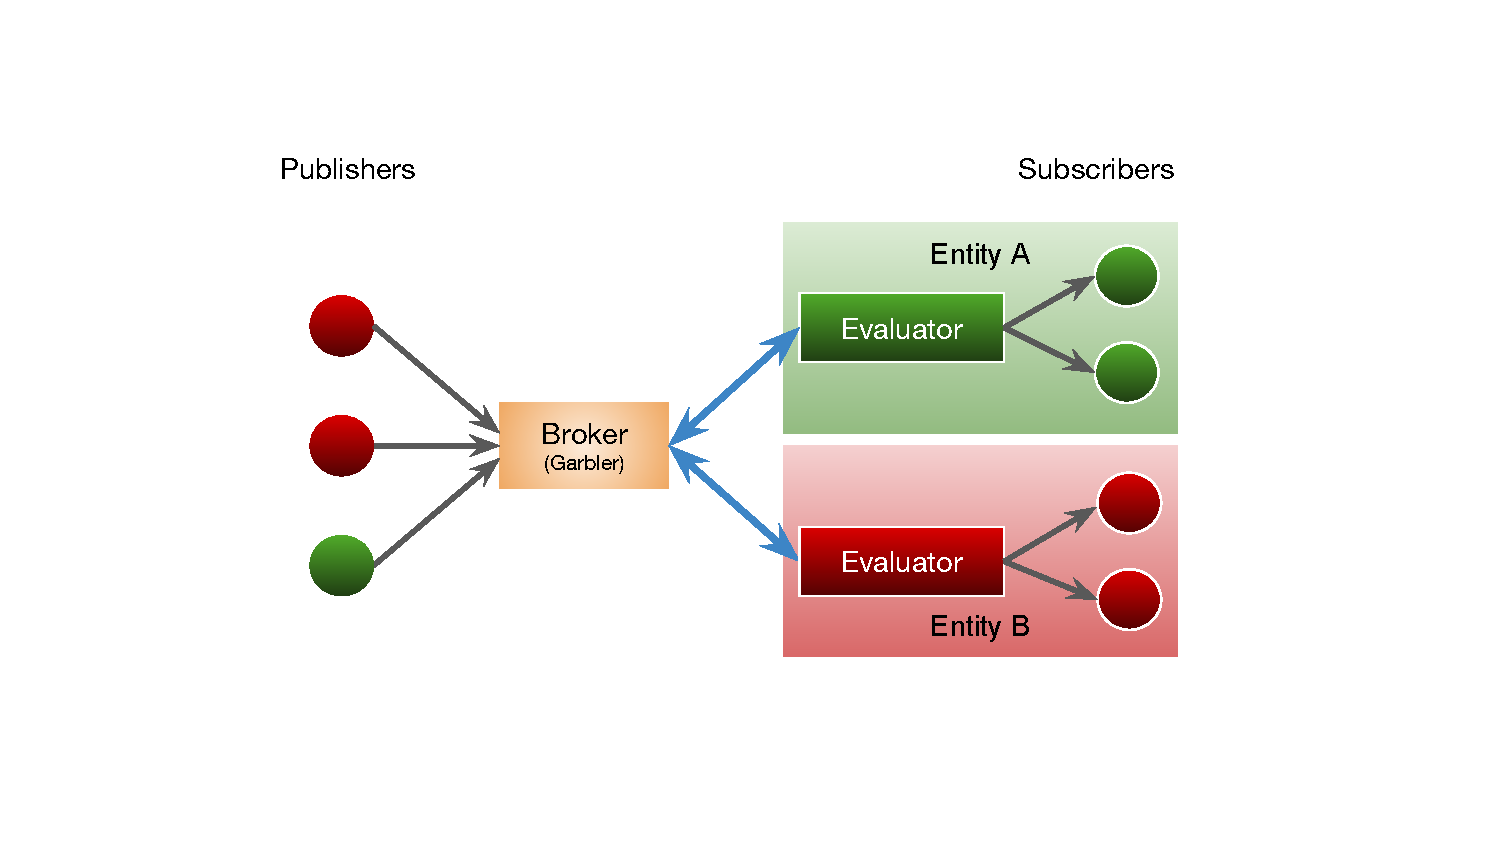
\includegraphics[width=0.95\textwidth]{figures/pps-local}
		\caption{Publish-Process-Subscribe setting with only a \broker, just like traditional topic-based publish-subscribe systems. This is suitable for large organization with several subscribers who can set up local computation. While we describe our protocol and system in the setting of Figure~\ref{fig:pps-out}, they can be easily adapted to this setting.}
		\label{fig:pps-local}
	\end{subfigure}

	\begin{subfigure}{0.45\textwidth}
		\centering
		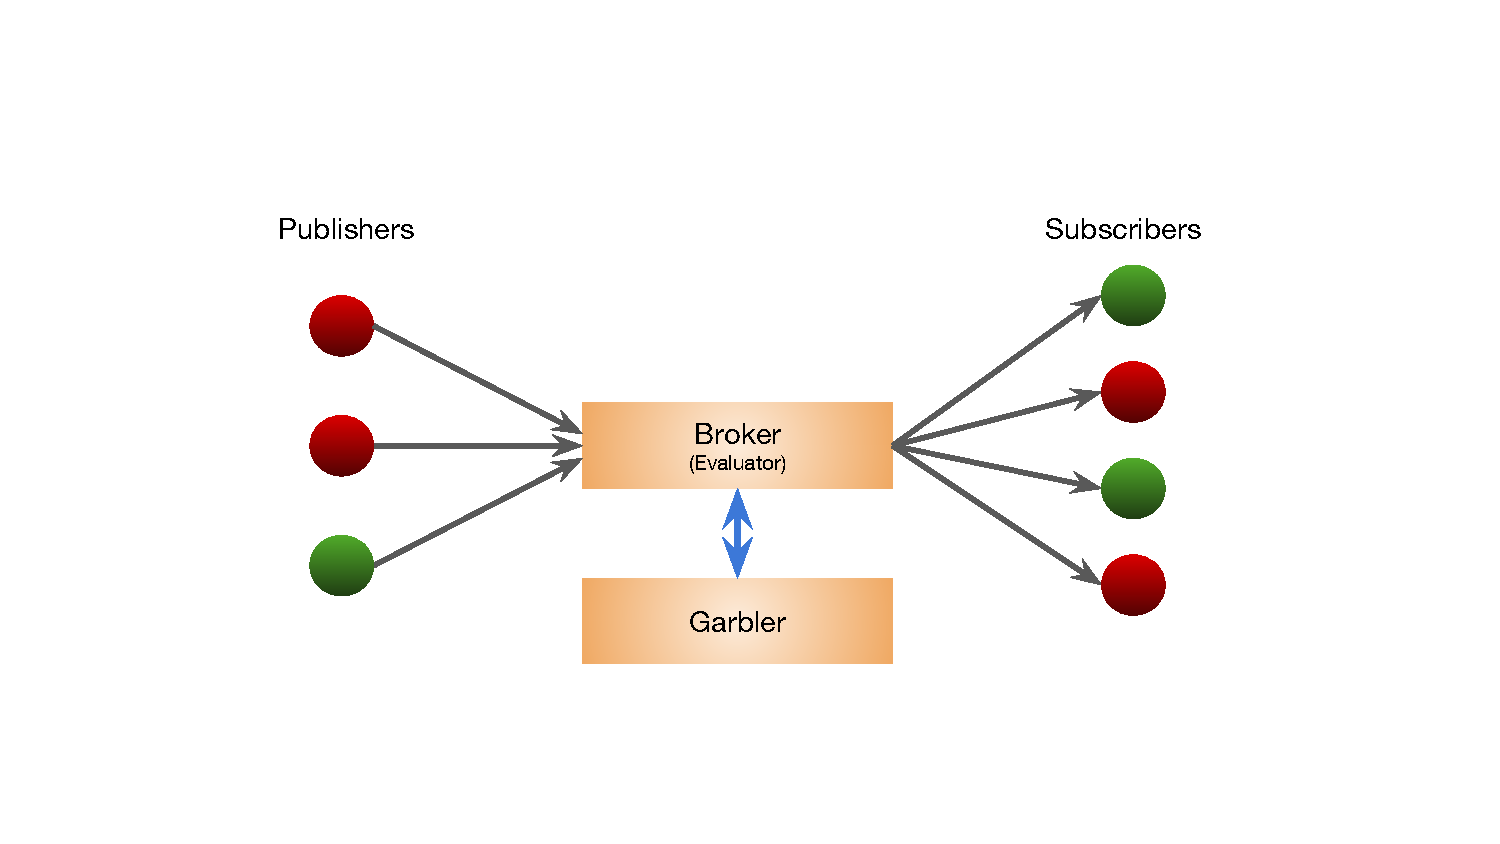
\includegraphics[width=0.95\textwidth]{figures/pps-out}
		\caption{Publish-Process-Subscribe setting with a separate entity, \garbler, to avoid expensive processing and communication at the subscriber's end. This is suitable for mobile devices. We describe our protocol and system in this setting.}
		\label{fig:pps-out}
	\end{subfigure}
	\vspace{12pt}
	\caption{Publish-Process-Subscribe System's Architecture}
	\label{fig:pps}
\end{figure}

\iffalse

The subscriber cannot compute it tehmselvds as they are using data from some
other entity, wihch may not want to share raw data.

\noindent\textbf{Publish-Subscribe}

\noindent\textbf{Garbled Circuits}

\noindent\textbf{Private-set-intersection (PSI)}

\fi


